\chapter{\label{app2:theory}Appendix: Click and connection through joint action}


Current research in joint action suggest that interoceptive predictive processes are at the core of successful human social interactions \citep{Graziano2013,Manera2013,Sparenberg2012,Springer2012}.  The essence of this proposal is that we use our own cognitive resources to build mental models of other people’s cognitions and the shared tasks that we share with others \citep{Tomasello2005a}.  Simulation of other people’s cognitive states (e.g., what they are feeling, thinking, and attending, a.k.a. a theory of mind) guide our expectations about their future behaviour, and in this way contribute to the viability of social interactions.



\section{Predictive coding\label{app2:predictiveCoding}}

PC first emerged as a data processing and compression strategy in computer science \citep{Rao1999}.  Researchers programmed a multi-layer artificial neural network to use downwards connections to match samples of .JPEG images with successful predictions. Visual signals were processed via a hierarchical system in which each level tried to predict activity at the level below it using recurrent feedback connections. If the feedback successfully predicted the lower-level activity, no further action was required. Failure of the model to predict the visual signal resulted in tuning and revision of the model using ``residual errors'' derived from the discrepancy between top-down predictions and lower-level activity.  Predictive coding offered a much more computationally efficient mechanism for data processing, because prediction errors were the only informational novelties in the system \citep{Clark2015}.



\section{Motor control\label{app2:motorControl}}
Successful regulation with the environment depends on an organism's capacity to move from its current state to a desired state.  In the case of the human evolutionary niche, organismic regulation hinges largely on movement, be it physical or simulated \citep{Wolpert1995}.

Theories of motor control generally agree the brain generates ``forward models'' that anticipate perceptual inputs and desired motor states \citep{Pickering2014}. The first paradigmatic theory of motor control suggested that forward models for action relied on special-purpose mechanism auxiliary to core mechanisms of perception of action \citep{Wolpert1997}.  This hypothesis, now known as the Auxiliary Forward Models \citep[AFM, see][]{Pickering2014}, relies on a dual mechanism of motor control.  First, a motor command is estimated in the brain by an ``inverse model,'' which contains as its inputs both the desired state and the actual state of the organism (e.g., the position of the body, see Figure ~\ref{fig:AFM}).  When the motor command is generated, an auxiliary copy (i.e., an ``efference copy'') is also generated, and is sent to a forward model which then generates predictions about action and perception by simulating the musculoskeletal system and contextual environment \citep{Wolpert1995,Blakemore1998,Flanagan2003}.  Prediction error arising from a discrepancy between predicted and resultant sensory inputs are then used as feedback to inform the generation of the next motor command in the inverse model, and so on in a loop, until the fit between sensory prediction and input is sharpened.

A more recent alternative proposal to the AFM suggests that forward models, instead of being auxiliary to, may instead lie at the heart of all forms of perception and action \citep{Friston2010}.  In contrast to AFM, the ``Integrative Forward Models'' account of motor control \citep[IFM, see][]{Pickering2014} posits that predictions from forward models act directly as action commands.  There is no dedicated mechanism used to predict the outcomes of our own (or others’) actions in addition to the action commands themselves.  Instead, generative action-oriented models are treated as the actual state of affairs, and cause a cascade of downward predictions about what should be the state of the models in the levels below (see Figure ~\ref{fig:IFM}).  In the IFM approach, there is no need for a motor command or efference copy at each level of action prediction, and prediction errors directly update the action models themselves.



\begin{figure}[htbp]
  \begin{center}
    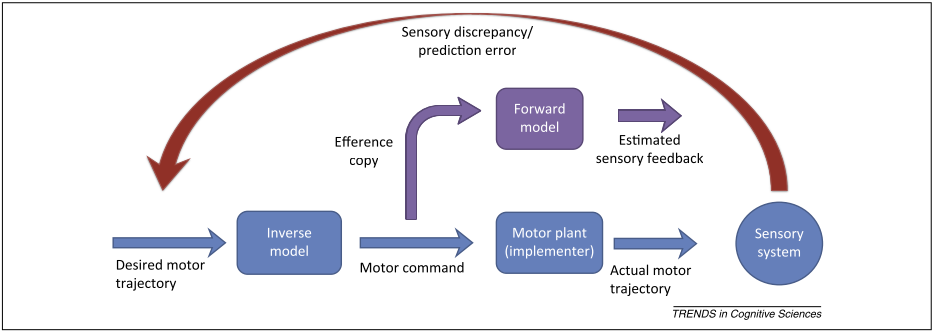
\includegraphics[scale=.4]{images/AFM.png}
      \caption{The Auxiliary Forward Model of motor control}
        \label{fig:AFM}
   \end{center}
\end{figure}

\begin{figure}[htbp]
  \begin{center}
    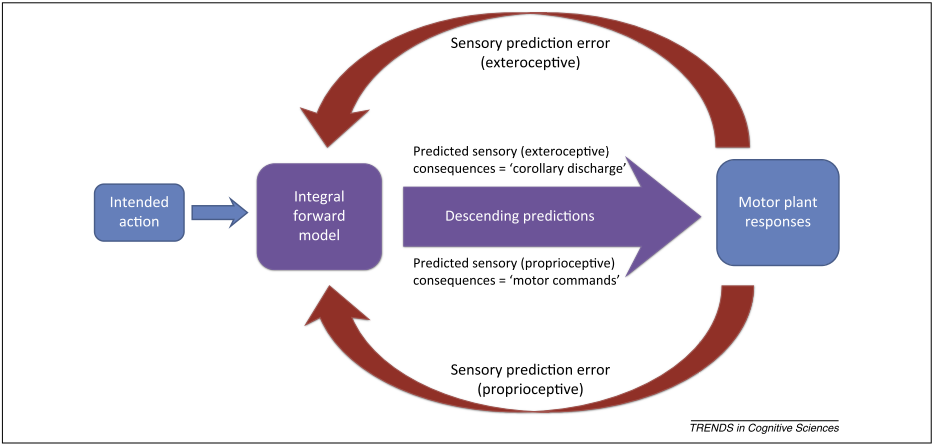
\includegraphics[scale=.4]{images/IFM.png}
      \caption{The Integrated Forward Model of motor control}
        \label{fig:IFM}
   \end{center}
\end{figure}


Both the AFM and IFM approaches agree that prediction, error minimisation, and hierarchical modelling are core processes in human cognition. From a thermodynamic standpoint, however, IFM appears to offer a more efficient model for free energy minimisation.  By replacing motor commands with direct predictions about proprioceptive and exteroceptive consequences, the need for a distinct optimal control calculation (i.e. an inverse model) disappears and along with it the need for an efference copy of the motor command, thus implicitly minimising various energetic costs \citep{Pickering2014,Friston2010}.   In place of the auxiliary mechanisms of the AFM, IFM posit a more complex (distributed) forward model mapping prior beliefs about desired trajectories to sensory consequences.  Whereas the ``heavy lifting'' in AFM required the use of an efference copy and inverse models, in IFM this work is done by the acquisition and use of a more complex predictive (generative) model \citep{Pickering2014}.

%According to the AFM account, the forward model is distinct from the inverse model, because it involves apparatus that computes the motor commands used to drive online action. Such a model is thus free to depart considerably in form from whatever governs the true kinematics of the agent.  Furthermore (in AFMs) the outputs of the forward model (i.e., the corollary discharge) do not cause movements – they are just used to finesse and predict outcomes and in learning.

%Comparisons between downward sweeps of prediction and upward sweeps of sensory input lead to a cascade of error signals throughout the hierarchy. These error signals are used to adjust the forward models that are guiding action execution (Clark, 2013). Importantly, actions are aimed at minimising prediction errors, by matching sensory inputs to predictions— a process termed active inference (Friston, 2008;Friston & Frith, 2015a, b). Eventually, active inference leads iteratively to a solution that will take the organism from its current motor state to the desired one.






\subsection{AIF in place of AFM}


%, which appear to be maximised in team click.

\subsubsection{AFM approach to joint action\label{app2:AFMapproachJA}}
 \textcite{Keller2016}, for example, presented a conceptual framework that applies an ``auxiliary forward model'' (AFM) approach to musical joint actions.  The AFM approach requires that agents produce models responsible for 1) individual action planning and control (self-internal models), 2) prediction of others' actions (other-internal models), and 3) representation of the shared goal (joint-internal models).  Of these three types of models, however, only self-internal models comprise the auxiliary predictive architecture (i.e., the forward model containing an efference copy of one's own action, and ``inverse models'' that are responsible for output of motor commands. See Appendix~\ref{app2:motorControl} for a more detailed explanation of these terms).  Thus, both anticipation and compensation in joint action depends on a control loop, whereby sensory information (error signals) are routed (fed-back) through self-internal models, which inform the production of auxiliary predictions---of self, other, and joint action---grounded in individual motor simulations.  Importantly, in this model,  error signals are fed-back only to the self-inverse model, as no inverse model for the joint action partner exists.

The now longstanding proposal that individuals only produce auxiliary predictive models of their own actions (as opposed to others' actions too) has served to explain how individuals effectively attend to others in joint action.  With privileged access to an efferent copy of impending individual action, an agent is able to preemptively attenuate sensitivity to their own action, in order to attend to the actions (and prediction errors) of others \citep{Wolpert1998}.  For example, the AFM approach provides an explanation for the phenomenon of tickling, or specifically why it is near impossible to tickle oneself \citep[due to sensory attenuation resulting from the self-generated predictions about the consequences of action][]{Blakemore2003}. However, while the AFM has proven adequate to explain individual motor control, and some instances of joint action (such as tickling), it also contains potential shortcomings when applied to dynamical joint action scenarios.

\textcite{Pesquita2017} summarise three shortcomings of an AFM approach to joint action.  First, the AFM model assumes a static and unchanging representation of the shared goal and the other's goal, and provides no mechanism through which the shared goal representation can be dynamically updated (based on prediction error signals).  This issue limits the ability of AFM to account for the real-world flexibility and interchangeability of shared goals (for example, the adaptive switching between the shared goal of carrying a table or the bench depending on the location of both objects).  Second, the same rigidity applies to other-inverse models.  The inability to directly and dynamically update other-models suggests the practical possibility that self and other models may gradually diverge over time due to the lack of sufficient predictive information regarding the actions of others \citep{Pickering2014}. Third, the AFM approach does not specify how sensory input is differentially used to update self and other models, which limits the model's ability to account for learning and adaptation within joint action \citep{Pesquita2017}.  Thus, not only does the AFM approach appear to be computationally intensive (due to the recruitment of auxiliary inverse models and dual motor commands, discussed in Section~\ref{sect:predictiveCoding}), it also appears to be unable to fully account for the dynamic interactive flexibility required of agents in real-world joint action.





%\myparagraph{Generalised synchronisation as a dynamical foundation for joint action}

\myparagraph{Precision-weighting self- and others}
In place of auxiliary processes of prediction, the AIF for joint action hinges instead on precision weighting of prediction errors in order to facilitate and finesse joint action \citep{Moutoussis2014,Friston2015}.  When engaged in joint action, the individual turns down the volume (reduce the precision weighting) on prediction errors relating to one's own action so that movement can occur unimpeded by over-attention to self-generated prediction errors \citep[an intuitive example of the opposite of this ideal scenario is a Skype call in which the flow of an individual's speech is interrupted by auditory feedback from the other receiver's device (feedback that would otherwise be attenuated by the speaker), see][]{Friston2015}.  Alternatively, when attending the the action of others, the attenuation of proprioceptive error signals can cease. In this way, precision weighting is used to flexibly adjust the volume of multi-modal prediction errors (exteroceptive, interoceptive, and proprioceptive) in order to finesse and sustain generalised synchronisation---the shared narrative on which joint action is sustained).

Heuristically, this suggests that active inference in joint action takes one of two modes; a ``sensory'' mode in which an agent flexibly attends to sensory inputs, or an ``active'' mode in which agents act and attenuate proprioception accordingly \citep{Friston2015}. To explain ticklishness, for example, the AIF can appeal to the ``sensory'' inferential mode in which the volume on proprioceptive prediction error is ``dialled-up.''  The failure of self-tickling, by contrast, can be explained as the product of an active mode of inference in joint action, in which the volume of proprioceptive prediction is ``dialled-down'' to enable smooth flow of action execution.
  \footnote{Recall also that instances of tickling commonly involve a stationary victim. While it indeed appears almost impossible to tickle oneself, it is also rare to be tickled while moving, i.e., acting during periods of sensory attenuation.}
Thus, the AIF approach to joint action depicts two or more brains constrained by dynamic coupling (general synchronisation), which model the sensory and perceptual predictions pertaining to the movement of self and others \citep{Pesquita2017}.


\subsection{Predictive Joint Action Model (PJAM)\label{sect:PJAM}}
 \textcite{Pesquita2017} have formulated a minimal architecture for an active inference approach to joint action, which they term a ``Predictive Joint Action Model'' (PJAM).  PJAM is comprised of three hierarchical levels of inference: goal representation, action-planning, and sensory routing (see figure ~\ref{fig:PJAM}).  Each level of the hierarchical model is informed by prediction errors from the level below, and the model works iteratively to minimise free energy in joint action scenarios.  In line with the AIF, PJAM does away with auxiliary processes of motor control and efferent copies, and posits instead that joint action emerges directly from two or more individuals reaching generalised synchronisation by converging on equivalent predictive models for joint action \citep{Friston2015}.

  \begin{figure}[htbp]
    \begin{center}
      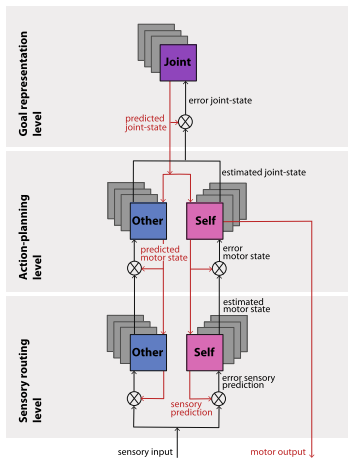
\includegraphics[scale=.8]{images/PJAM.png}
        \caption{The Predictive Joint Action Model \citep{Pesquita2017}}
          \label{fig:PJAM}
     \end{center}
  \end{figure}

In contrast to the AFM approach, which posits a shared goal representation deriving from self-internal models, the PJAM suggests that a shared goal derives primarily from the dynamical coupling of agents to each other and to other (shared) affordances of the task-specific environment (generalised synchronisation).  Thus, rather than being wholly explicit, propositional, or pre-set, the shared goal is understood to span the entire predictive hierarchy, with basal coupling of sensorimotor processes at the lower end, through to more elaborate and flexible models that facilitate more explicit or propositional correlations, at the higher end.  In a bidirectional cascade of prediction and prediction error, the ``shared narrative'' at the goal representation level generates discrete action plans for self and other, which are then tested against prediction errors arising from the sensory routing models below \citep{Pesquita2017}.

\subsubsection{Evidence in support of PJAM}
PJAM (and the AIF which it extends) predicts that joint action will be established and maintained through generalised synchronisation between two or more predictive brains driven by an overarching mandate of free energy minimisation \citep{Friston2015}.  In particular, PJAM predicts that co-actors in joint action will generate predictive models that reflect 1) a shared goal, 2) action plans for self and other, and 3) routing instructions for sensory inputs.  Consistent with the modelling view of the AIF (see Section~\ref{sect:thermoCog}), these three layers of generative models will reflect an hierarchy of complexity, and will be coupled to a continuum of natural and conventional affordances.  Below I outline existing experimental evidence in support of these predictions.





\myparagraph{Evidence for self and other action plans}
On the level of self and other action plans, experimental evidence suggests that co-actors generate internal models of self and other either spontaneously and involuntarily---as in the commonly used social simon task experimental paradigm \citep{Sebanz2003,Atmaca2008}---or more deliberately---as in a coordinated dyadic horizontal jumping task \citep{Vesper2012}.  \textcite{Loehr2016} demonstrate that when learning a joint piano piece, musicians are able to better perform a piece together rather than solo, which suggests that representations about each participant in joint action are encoded within the joint context of the interaction.
Studies also show that the capacity for co-representation of self and other action plans is modulated by mood \citep[positive or negative affect, see][]{Kuhbandner2010}, self-concept and social orientation \citep{Colzato2012,Colzato2012a}, and processes of group membership \citep{DeBruijn2008,Aquino2015}. This evidence lends support to the proposal that active inference involves coupling with various natural and conventional affordances in order to flexibly integrate information deriving form various sensory inputs.


\myparagraph{Evidence for sensory routing}
On a sensory-routing level, evidence suggests that modulation in sensory attenuation is driven by the predictability of the outcome, as opposed to necessarily being driven by the presence or absence of auxiliary efference copies \citep{Sato2008}.  In addition, attributing sensory consequences to joint action partners is linked to cooperative success \citep{Chaminade2012}, suggesting that finely tuned sensory routing based on predictions of self and other actions could be key to successful coordination.





















\subsection{PJAM\label{app2:PJAM}}

PJAM assumes that each participant in a joint-action maintains internal models of 1) the joint task, 2) the action contributions of self and others to the joint task, and  3) the sensory-motor inputs expected from action plans.

The \textit{goal-representation} level of PJAM suggests that participants in joint action generate and monitor representations of the shared task. This proposal is formulated from evidence that musicians maintain shared representation of desired unified sound of an ensemble \citep{Keller2008}.  In one study, for example, Loehr and colleagues  use a neurophysiological measurement that codes unexpected events (ERP) to show that musicians tracked deviations from a desired joint state \citep{Loehr2013}; in another study, Loehr and Vesper \textcite{Loehr2016} demonstrated that playing music together generates shared expectations regarding the desired state of joint action, and this process guides future action.  Taken together, this evidence suggests that participants in joint action utilise prediction errors arising from lower levels to update representations of shared tasks.  The key point here is that joint action is facilitated by embodied and inactive predictions of a shared task, and not just auxiliary predictions about an individual's role in shared processes, as an AFM approach would suggest \citep{Keller2016}.
%(Wolpert MOSAIC model doesn't account for updating rep. of shared task)


At the \textit{action-planning} level of PJAM, pairs of models predict the contributions of self and others to a joint action.  The ``shared narrative'' at the goal representation level generates discrete action plans for self and other, which are then tested against prediction errors arising from the sensory routing models below \citep{Pesquita2017}.  This level of PJAM is supported by evidence that participants in joint action generate internal models of self and other, known as co-representation, either spontaneously and involuntarily, as in the commonly used social simon task experimental paradigm \citep{Sebanz2003,Atmaca2008}, or more deliberately, as in a coordinated dyadic horizontal jumping task \citep{Vesper2012}.

Action-planning entails, on the highest level, action roles; on a mid-level, movement trajectories; and on the lowest level, movement of muscle groups of self and others \citep{Pesquita2017}.  As with goal representation, action-planning for self and others is a predictive process \citep{Flanagan2003}, in which individuals encode motor predictions and resulting errors of others' actions in addition to their own \citep{VanSchie2004,Radke2011}.  Predictive models of self and other action plans appear to be grounded in an individual's own motor simulation processes, such that each participant maintains covert motor activations relating to expected contributions of their partners \citep{Hollander2012}.  This evidence serves to directly challenge the AFM approach to joint action, which suggests that individuals only generate self-focussed forward models for prediction.

There is evidence to suggest that motor simulation of self and other action plans is mediated by the existence of a shared goal between co-actors \citep{Kourtis2010}.  \textcite{Loehr2016} demonstrate that when learning a joint piano piece, musicians are able to better perform the piece together rather than solo, which suggests that representations about each participant in joint action are encoded within the joint context of the interaction.  In other words, when we learn a joint task we not only learn our own role, but also the impact of other's roles on our own role in the joint action.

In sum, the action planning level of PJAM proposes that models of the self and models of partners can be paired to represent the possible combinations of individual contributions to the joint action. These models transform the desired joint-state signal, descending from the goal representation level, into expectations of the unique motor states of the self and the partner.  Error signals arrive from levels of the model below, with sensory routing.  Studies also show that co-representation is modulated by mood \citep[positive or negative affect, see][]{Kuhbandner2010}, self-concept and social orientation \citep{Colzato2012,Colzato2012a}, and group membership \citep{DeBruijn2008,Iani2013}.

The \textit{sensory routing} level receives the inflow of sensory input and compares it to internal model predictions pertaining to each participant's action outcomes on the level above.  This comparison process serves as a gate for parsing sensory information into their corresponding predictive streams (self or others, see Figure ~\ref{fig:PJAM}). This process allows the predictive system to attribute external consequences to each individual’s actions.   For example, two people carrying a table will receive haptic input from the table. This input will be confounded with respect to its source, in that the haptic input itself does not differentiate between the forces that each brother applies to the table. However, the comparison between the haptic input and the separate predictions about one’s own and the other’s action will help feed each predictive cascade of self and other into their respective streams \citep{Pesquita2017}.

Consistent with other levels of PJAM, deviations between sensory input and sensory predictions (i.e., prediction errors) are fed-back to sensory predictive models in order to continuously improve sensory parsing.  As foreshadowed above, evidence indicates that accurate prediction of others' actions is associated with the attenuation of sensorial experience of joint action outcomes.  Predictions about motor outcomes are used to filter out the sensory feedback produced by the same action \citep{Blakemore1999}.  This proposal is confirmed by evidence that greater sensorial experience occurs when an outcome is unexpected, as opposed to predicted from prior self or other action \citep{Sato2008}.  In addition, attributing sensory consequences to joint action partners is linked to cooperative success \citep{Chaminade2012}, suggesting that finely tuned sensory routing based on predictions of self and other actions could be key to successful coordination.

\subsection{Dynamic coupling in joint action\label{app2:dynamicCoupling}}

One main prediction of the AIF for joint action, if it is correct, is that joint action will exhibit properties of dynamical systems.  In particular, it should be possible to identify coupling of system component degrees of freedom in joint action \citep{Turvey1978,Schmidt1990}.  Dynamic coupling can be identified by two core properties:  1) dimensional compression (potentially independent DF are coupled so that the synergy possesses a lower dimensionality than the set of components from which it arises) and 2) reciprocal compensation (the ability of one component of a synergy to react to changes in others) \citep{Riley2011}.  Indeed, an accumulation of evidence has identified the existence of functional synergies on multiple levels of human behaviour, from brain function \citep{Yufik1998,Sengupta2013}, to interpersonal interactions \citep{Kelso2009,Riley2011,Fusaroli2014}, to large-scale human societal dynamics \citep{Nowak2017}.

In the case of joint action in particular, individuals have been found to couple and reciprocally constrain their movements reducing the overall control needed to maintain effective cooperation \citep{Ramenzoni2011,Ramenzoni2012,Riley2011,Schmidt1990}.  Individuals’ behaviours become increasingly interdependent, so that a higher-level structure of the interaction emerges.

%This kind of emerging organisation has previously been referred to as soft-assembly \citep{Kello2009}: individuals preserve a degree of autonomy, but their behaviour is constrained by the interaction. They can flexibly engage and disengage from it, as well as become part of other soft-assemblies \citep{DeJaegher2010,DiPaolo2012}.

Research into the coordination dynamics of real-world joint actions  has shown evidence of dynamic coupling in joint-action tasks, such as dancing, martial arts, and moving objects like furniture.  In these studies, specific component degrees of freedom are modelled as coupled oscillators \citep[using the HKB model, which describes the change in the relative phase between two oscillatory components.   See][]{Haken1985,Kelso1986}.  Models are analysed for non-random fluctuations in relative phase over multiple time scales.  This type of synchronisation is said to be of a fractal or semi-fractal organisation, also known as 1/f scaling or ``pink noise'' \citep{Caron2017}.  According to Anderson and colleagues \citep{Anderson2012}, 1⁄f scaling is ubiquitous in smooth cognitive activity, and indicates a self-similar structure in the fluctuations that occur over time (within a time series of measurements).
1⁄f scaling indicates that the connections among the cognitive system's components are highly nonlinear \citep{Ding2002,Holden2013,Kello2010,Riley2011,VanOrden2003,VanOrden2005}. Interestingly, pink noise has been measured beyond dyadic synchronisation, in the analysis of sub-phases of team sports \citep{Passos2014,Duarte2012} and group dancing \citep{Chauvigne2017}.
  \footnote{1⁄f scaling is temporal long-range dependencies in the fluctuations of a repeatedly measured behaviour or activity. Analogous to spatial fractals, 1⁄f scaling denotes a fractal or self-similar structure in the fluctuations that occur over time. That is, higher frequency, lower amplitude fluctuations are nested within lower frequency, higher amplitude fluctuations as one moves from finer to courser grains of analysis \cites(for a more detailed description see, for example)(){Holden2005}{Kello2009}.}

In addition to the pink noise of dynamic coupling in joint action, research has also attempted capture movement signatures of joint action that resemble instances of ``identical synchronisation,'' or the idea of being ``in the zone'' with a co-actor.  Working within the common dyadic ``mirror game'' paradigm, Noy and colleagues \textcite{Noy2011,Noy2015,Hart2014} have developed an experimental proxy for an optimal state of togetherness in joint action.  ``Co-confident motion'' (CC motion) is canonical movement pattern of synchronised motion characterised by smooth and jitter-less motion, without the typical jitter resulting from reactive control in more commonly encountered leader-follower patterns.  In CC motion, different players appear to shift their basic motion signatures to a movement shape that is altogether different from their individually preferred shapes \citep{Hart2014}. Importantly, the pattern of CC motion shares the same sine wave shape as the optimal solution of the minimum jerk model, a well-known motor control model for rhythmic motion \citep{Hogan2007}.

Noy and colleagues suggest that it is possible that during CC motion periods of joint action, two players converge to a canonical pattern stemming from an optimal state of each participant’s motor control system.  The resulting motion may be easier to predict and to agree on. Furthermore, participants appear to use smooth elementary strokes of CC motion as the building blocks for more complex motion \citep{Noy2017}.  This observation raises the possibility that CC motion, a state of alignment in which individual components converge in a transcendent, functional synergy, could set the cognitive foundation for more efficient and effective higher level processes of communication and information transfer \citep[15]{Lerique2016}.  This evidence accords with the proposal that joint action is underwritten by the fact that two or more agents share functionally and formally equivalent ``shared narrative'' that transcend self and other agency, and instead involve a ``we'' mode of social cognition \citep{Gallotti2013}.

In support of this line of research, experimental evidence has shown that functional interpersonal synergies (dynamic coupling) facilitate performance of social cognitive or linguistic tasks, such as gaze coordination and turn taking in conversation \citep{Miles2010,Richardson2005,Shockley2009}.  Conversely, being psychologically distanced from another individual can inhibit the emergence of interpersonal synergies \citep{Miles2010}.

%The ways in which dynamic coupling between coactors facilitate adaptive information transfer between individuals and within groups suggests that psychological mechanisms and cultural practices responsible for generating these synergies could have been subject to cultural evolutionary forces of selection and attraction \citep{Claidiere2014,Mesoudi2016a}.


\subsubsection{Action-perception links in joint action\label{app2:actionPerceptionLinks}}

Evidence of dynamic coupling between co-actors in joint action is further bolstered by parallel strands of research in psychology \citep{Prinz1990,Prinz1997,Prinz2013}, neurophysiology \citep{Rizzolatti2004,Rizzolatti2010}, and neurocognition \citep{Wolpert1998,Wolpert2000} that interpersonal behavioural coordination in joint action is facilitated by the intrinsic coupling—--under certain circumstances---of action perception and action execution in the human brain.

Since Prinz’s (1990) initial proposal that perception and action are coded in a common representational domain, and are therefore linked by shared neural resources, research into action-perception coupling has spanned individual action as well as interpersonal social interaction.
In terms of its function for joint action scenarios, action-perception coupling is regarded as a basic link between sender and receiver that provides procedural, perceptual, and emotional common ground between individuals \citep{Rizzolatti1998}.

In essence, action-perception coupling refers to the ostensive co-occurrence of a stimulus for action and its motor representation.  For example, the representation of a perceptual effect (say the sound of a middle-C on a piano) can trigger the movement necessary to produce the effect itself (motor instructions for playing the middle-C key on a piano).   Importantly, evidence suggests that sensory-motor coupling emerges primarily as a result of motor learning: having only visual \citep{Candidi2014} or auditory \citep{Lahav2007} experience with a given action is not sufficient to trigger these motor responses—--active motor learning is necessary.  As such, most research into action-perception coupling occurs with individuals who have mastered a certain sensorimotor task, such as expert musicians, whose movements and intended sounds become strongly associated \citep{Novembre2014}.

In behavioural experiments in which samples of musicians are compared to non-musician controls, researchers demonstrate that auditory perception primes action if strong action-perception links have been established through instrument-specific training \citep{Drost2005,Drost2005a,Drost2007}.  For example, Drost and colleagues showed that sound cues incongruent with the prescribed action response (the sound cue of a D chord when the prescribed action response is a C chord) delayed execution time \citep{Drost2005} and induced more false responses \citep[i.e., production of the heard chord, instead of the imperative one,][]{Drost2005a} in pianists but not non-pianists.  \textcite{Keller2006} showed that mental images of anticipated action effects can prime responses to a similar degree as is observed with congruent and incongruent sounds, highlighting the role of action-perception coupling in action preplanning (i.e., before sounds are actually perceived).  Further studies demonstrated that action-perception coupling does not only enhance the efficiency of action planning, but also facilitates timing accuracy and economical force control by optimising movement kinematics \citep{Keller2010}.

Neurophysiological evidence suggests a neural signature for action-perception coupling in the motor cortices.  Haueisen and Knosche \citep{Haueisen2001} conducted a magnetoencephalography (MEG) study (of piano players with and without experience) and showed that perception of piano pieces led to an increase of neural activity over the motor cortex hand area in piano players but not non-musicians.  Bangert and colleagues \textcite{Bangert2006} ran an fMRI study where professional pianists and non-musicians heard novel piano sequences that were synthesised online (and therefore could not be familiar).  Compared to non-musicians, professional pianists showed a broad network of motor areas responding to the piano sequences, including both primary motor and premotor (BA 4/6) regions.  Besides auditory- and visual-motor coupling, tactile, proprioceptive and haptic sensory feedback has been shown to induce coupling \citep{Schulz2003,Kuchenbuch2014}.

These behavioural and neurophysiological data, taken together, indicate that musical training leads to the emergence of cross-modal action-perception coupling, where perception of the effects of musical actions (either the sounds produced or the visual presentation of the movement patterns) triggers proprioceptive predictions for the movements necessary to produce these effects. Interestingly, these effects have also been observed in trained non-experts \citep{Bangert2003,Lahav2007}.  Lahav and colleagues (2007), for example, trained non-musicians to play a piano piece by ear (without notation) over a period of five days and found that activation of the frontoparietal motor-related network (comprising Broca’s area, the premotor region, the intraparietal sulcus, and the inferior parietal region) increased most strongly for the trained pieces, versus untrained (but motorically known) and familiar but motorically unknown pieces.

It has been argued that the function of action perception coupling is twofold.  First, coupling of this nature supports a neurophysiological capacity to anticipate our own as well as other's  (i.e., observed) actions.  \textcite{Maidhof2009} and \textcite{Ruiz2009} conducted two similar EEG studies in which they examined the ERPs preceding the execution of piano errors in pianists and non-musicians.  In pianists (but not non-musicians) errors were detected prior to their execution (the EEG signal was found to anticipate the actual mistake by 100 ms \citep{Maidhof2009} and 50–70 ms \citep{Ruiz009}.  These data thus indicate that the coupling of sensory and motor cortices has a strong anticipatory function that, given the existence of an association between movements and their ensuing effects, permits the generation of predictions about the state of our own body and the sensory consequences of our movements.

Second, action-perception links act as a resource for the co-representation of and coordination with others in joint action.
Research demonstrates that the training-mediated coupling of perception and action is not confined to individual behaviour.  As mentioned above, there is evidence to suggest that expert ensemble musicians form representations of self and other-related actions, and that these representations are influenced by properties of the individual’s own motor system \citep{Novembre2012}.  Action-perception links can be used for monitoring and integrating (e.g., timing or combined pitches) the actions of other ensemble members with self-generated actions \citep{Loehr2013}, and these effects appear to be stronger in individuals with high perspective taking skills \citep{Novembre2012,Loehr2013}.  The overlap between mechanisms for action production and action observation suggests that individuals may represent their own and others’ actions in a commensurable format.  Training-induced motoric representation of self and other actions may facilitate various capacities important for joint action, such as prediction, adaptation, and entrainment.

These various strands of research, when recast in an active inference paradigm, can be understood as evidence for the role of Bayesian precision-weighting of error-signals for the optimisation of performance in joint action.  Tight coupling between action and perception in expert practitioners indicates high precision weighting of interoceptive and proprioceptive prediction errors.   According to PJAM, tight coupling of perception and action is the result of an iterative learning process in which individuals develop a ``grasp'' of a 1) shared narrative for action, 2) predictions concerning the action plans of self and other, and 3) routing of exteroceptive, proprioceptive, and interoceptive prediction error signals.  In other words, this grasp in joint action is equivalent to the optimal reduction in free energy across multiple hierarchical layers of prediction in the brains of each co-actor.

%Explain with AFM is not the best model for explaining action-perception links
\subsubsection{The utilisation of extrapersonal resources in joint action\label{sect:rowerStudy}}
A recent field study by R'Kiouak and colleagues (2016) supported this line of reasoning.  Through combined analysis of phenomenological and video data derived from a close study of two unacquainted expert rowers who participated in a real world dyadic rowing exercise (coxless pair), the authors found that athletes reported joint action as being salient and meaningful only 24.5\% of the race under study (e.g., during synchronisation breakdowns), whereas the rowers did not pay attention to the effectiveness of their joint action for the remaining 75.5\% of the studied period \citep{RKiouak2016}.  In other words, these results suggest that the rowers were able to coordinate their strokes through experiencing their joint action as meaningless during a large part of their joint activity.  These results lead the authors to suggest that extra-personal regulation processes might have underlain the dynamics of the joint action, such that athletes used the environment to mediate the arrangement of individual and joint activities. This corroborates that team coordination patterns of movement may occur without a perfectly shared experience about the ongoing joint action \citep{Bourbousson2011,Bourbousson2012}. The study provides evidence that the full coordination of sense-making activities is not needed to allow for a viable patterned joint action in a natural task, as long as actors are simultaneously involved in co-regulating their collective behaviour \citep{Froese2011,Froese2014}.
The authors interpret the results as evidence for a ``stigmergic'' theory of collective behaviour \citep{Susi2001,Avvenuti2013}, in which holistic phenomena of coordination might be considered as emerging from the behaviour–environment coupling.


















%%%%%%%%%%%%%%%%%%%%%%%

\subsection{General synchronisation in joint action\label{sect:generalSync}}
\subsubsection{Direct coupling deriving from general synchronisation in joint action}

  An active inference approach to joint action is grounded in thermodynamic cognition and dynamical systems theory \citep{Friston2013}.  Friston and Frith point out that generalised synchronisation is an inevitable and emergent property of coupling two systems that are trying to predict each other ~\ref{Friston2015}.  Generalised synchrony refers to the synchronisation of chaotic dynamics \citep{Barreto2003}.  The basic principle is as follows.  If the universe comprised two biological (free energy minimising) systems---you and me---then your states and my states have to be restricted to an attracting set of states that is small relative to all possible states we could be in \citep{Friston2015}.  This attracting set of states enforces a generalised synchrony in the sense that the state you are in imposes constraints on states I occupy \citep{Richardson2015}.  It is in this sense that generalised synchronisation is a fundamental aspect of coupled dynamical systems that are free energy minimising.  If we are both trying to minimise the free energy of our attracting set (by reducing surprise or entropy), then synchronisation will be more manifest \citep{Friston2015a}.

In the case of the cognition of joint action, generalised synchronisation can be understood as the level of interdependence between levels of hierarchical models generated by two more (Bayesian) brains.  Friston and Frith call this the ``shared narrative'' that enables joint action.  Within general synchronisation, ``identical synchronisation'' refers a moment in which two or more models show identical equivalence between each hierarchical layer of prediction \citep{Friston2015}.   In contrast to behavioural synchrony, general synchronisation refers to alignment on a cognitive (information-theoretic) level, as opposed to merely a behavioural level. Behavioural synchrony may indeed suggest underlying cognitive synchronisation, either general or identical.
